\documentclass[tikz]{standalone}
\usepackage{tikz}
\usepackage{amsmath}
\usetikzlibrary{calc}
\usetikzlibrary{positioning}
\usetikzlibrary{fit}
\usetikzlibrary{backgrounds}
\usetikzlibrary{shapes.geometric}

\definecolor{lightGreen}{HTML}{d5e8d4}
\definecolor{lightYellow}{HTML}{fff2cc}
\definecolor{lightGray}{HTML}{f5f5f5}
\definecolor{lightRed}{HTML}{ff9999}
\definecolor{lightBlue}{HTML}{d5e5fc}
\definecolor{lightCyan}{HTML}{a7dfe3}
\pgfdeclarelayer{main_bg}
\pgfdeclarelayer{back_bg}
\pgfsetlayers{main_bg,main}


\newcommand{\mem}[2]{
    \begin{scope}
        \node (#1) [draw, rectangle, text width=\cellWidth, minimum width=\cellWidth*8, minimum height=\cellHeight, #2] {};
        \node (#1_cell_0) [draw, rectangle, text width=\cellWidth, minimum width=\cellWidth, minimum height=\cellHeight, right=0.0pt of #1.west, anchor=west] {};
        \foreach \x in {1,...,7} {
            \pgfmathtruncatemacro{\prev}{\x-1}
            \node (#1_cell_\x) [draw, rectangle, text width=\cellWidth, minimum width=\cellWidth, minimum height=\cellHeight, right=-\the\pgflinewidth of #1_cell_\prev] {};
        }
    \end{scope}
}

\begin{document}
    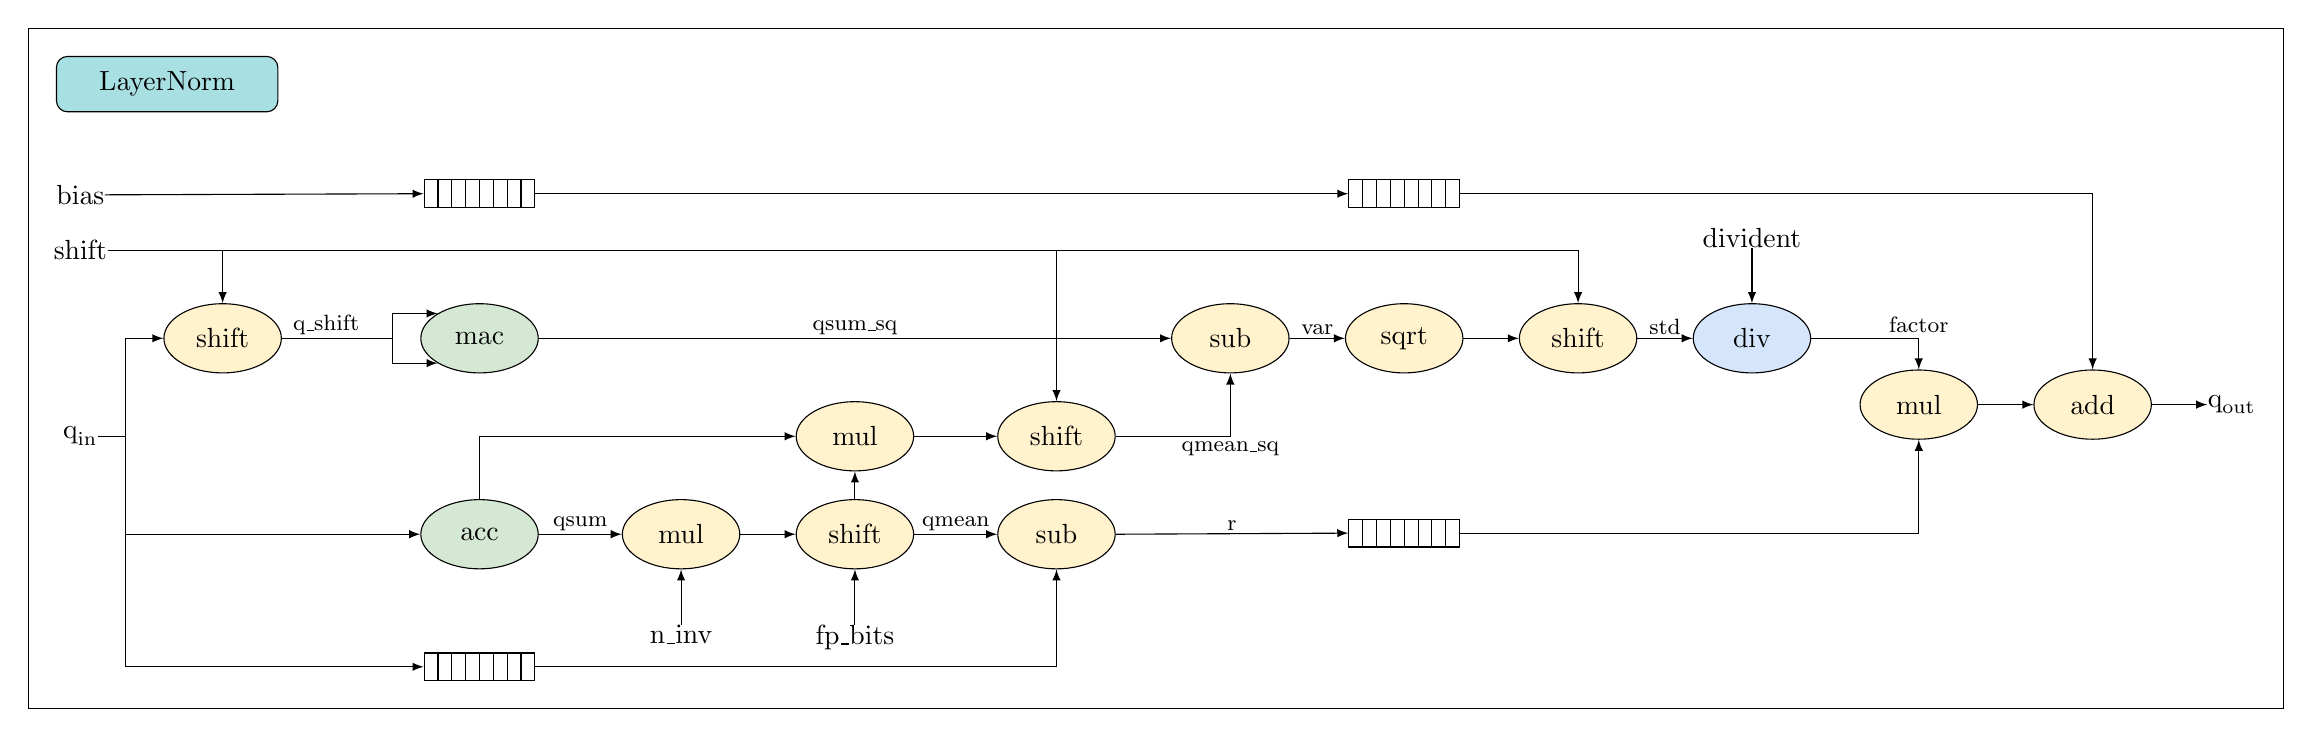
\begin{tikzpicture}[inner sep=0.0 pt, align=center]
    \pgfmathsetmacro{\rectWidth}{40}
    \pgfmathsetmacro{\rectHeight}{40}
    \pgfmathsetmacro{\ellWidth}{30}
    \pgfmathsetmacro{\ellHeight}{25}
    \pgfmathsetmacro{\cellWidth}{5}
    \pgfmathsetmacro{\cellHeight}{10}

    
    \node (qin) {$\text{q}_{\text{in}}$};
    \node (d) [ellipse, text width=\ellWidth, minimum width=\ellWidth, minimum height=\ellHeight, right=\rectWidth*0.75pt of qin.center] {};
    \node (d1) [ellipse, text width=\ellWidth, minimum width=\ellWidth, minimum height=\ellHeight, right=\rectWidth*0.5pt of d] {};
    \node (bias) [above=\rectWidth*2pt of qin] {bias};
    \node (shift) [above=\rectWidth*1.5pt of qin] {shift};
    \node (d2) [ellipse, text width=\ellWidth, minimum width=\ellWidth, minimum height=\ellHeight, below=\rectWidth*0.25pt of d] {};
    \node (acc) [draw, ellipse, fill=lightGreen, text width=\ellWidth, minimum width=\ellWidth, minimum height=\ellHeight, right=\rectWidth*1.25pt of d2] {acc};
    \node (mean) [draw, ellipse, fill=lightYellow, text width=\ellWidth, minimum width=\ellWidth, minimum height=\ellHeight, right=\rectWidth*0.75pt of acc] {mul};
    \node (mean_sh) [draw, ellipse, fill=lightYellow, text width=\ellWidth, minimum width=\ellWidth, minimum height=\ellHeight, right=\rectWidth*0.5pt of mean] {shift};
    \node (sub) [draw, ellipse, fill=lightYellow, text width=\ellWidth, minimum width=\ellWidth, minimum height=\ellHeight, right=\rectWidth*0.75pt of mean_sh] {sub};
    \node (meansq) [draw, ellipse, fill=lightYellow, text width=\ellWidth, minimum width=\ellWidth, minimum height=\ellHeight, above=\rectWidth*0.25pt of mean_sh] {mul};
    \node (sum_sh) [draw, ellipse, fill=lightYellow, text width=\ellWidth, minimum width=\ellWidth, minimum height=\ellHeight, right=\rectWidth*0.75pt of meansq] {shift};
    \node (d2) [ellipse, text width=\ellWidth, minimum width=\ellWidth, minimum height=\ellHeight, above=\rectWidth*0.25pt of sum_sh] {};

    \node (qinshift) [draw, ellipse, fill=lightYellow, text width=\ellWidth, minimum width=\ellWidth, minimum height=\ellHeight, above=\rectWidth*0.25pt of d] {shift};
    \node (mac) [draw, ellipse, fill=lightGreen, text width=\ellWidth, minimum width=\ellWidth, minimum height=\ellHeight, right=\rectWidth*1.25pt of qinshift] {mac};
    \node (var) [draw, ellipse, fill=lightYellow, text width=\ellWidth, minimum width=\ellWidth, minimum height=\ellHeight, right=\rectWidth*0.5pt of d2] {sub};
    \node (sqrt) [draw, ellipse, fill=lightYellow, text width=\ellWidth, minimum width=\ellWidth, minimum height=\ellHeight, right=\rectWidth*0.5pt of var] {sqrt};
    \node (std_sh) [draw, ellipse, fill=lightYellow, text width=\ellWidth, minimum width=\ellWidth, minimum height=\ellHeight, right=\rectWidth*0.5pt of sqrt] {shift};
    \node (div) [draw, ellipse, fill=lightBlue, text width=\ellWidth, minimum width=\ellWidth, minimum height=\ellHeight, right=\rectWidth*0.5pt of std_sh] {div};
    
    \node (mul) [draw, ellipse, fill=lightYellow, text width=\ellWidth, minimum width=\ellWidth, minimum height=\ellHeight, below right=\rectWidth*0.15pt and \rectWidth*0.75pt of div] {mul};
    \node (add) [draw, ellipse, fill=lightYellow, text width=\ellWidth, minimum width=\ellWidth, minimum height=\ellHeight, right=\rectWidth*0.5pt of mul] {add};
    \node (qout) [right=\rectWidth*0.5pt of add] {$\text{q}_{\text{out}}$};
    \node (const) [above=\rectWidth*0.5pt of div] {divident};
    \node (fp_bits) [below=\rectWidth*0.5pt of mean_sh] {fp\_bits};

    \node (const1) [below=\rectWidth*0.5pt of mean] {n\_inv};
    
    \draw (bias -| mac) node [name=bias1_mem_pos, text width=\cellWidth, minimum width=\cellWidth, minimum height=\cellHeight] {};
    \mem{bias1_mem}{below=-\the\pgflinewidth of bias1_mem_pos.north, anchor=north}
    \mem{acc_mem}{below=\rectWidth*0.75pt of acc}

    \draw (sub -| sqrt) node [name=div_mem_pos, text width=\cellWidth, minimum width=\cellWidth, minimum height=\cellHeight] {};
    \mem{div_mem}{below=-\the\pgflinewidth of div_mem_pos.north, anchor=north}
    \draw (bias -| sqrt) node [name=bias2_mem_pos, text width=\cellWidth, minimum width=\cellWidth, minimum height=\cellHeight] {};
    \mem{bias2_mem}{below=-\the\pgflinewidth of bias2_mem_pos.north, anchor=north}

    \node [draw, fill=lightCyan, rounded corners, minimum width=\rectWidth*2, minimum height=\rectHeight*0.5, above=\rectWidth*1pt of bias.west, anchor=west] (layernorm) {LayerNorm};

    \draw [-latex] (qin.east) -| ([xshift=\rectWidth*0.25pt]qin.east) |- (acc_mem.west);
    \draw [-latex] (qin.east) -| ([xshift=\rectWidth*0.25pt]qin.east) |- (acc.west);
    \draw [-latex] (acc.east) -- (mean.west) node[midway, above, yshift=1pt, font=\footnotesize] {$\text{qsum}$};
    \draw [-latex] (qinshift.east) -| ([xshift=\rectWidth*1pt]qinshift.east) node[pos=0.2, above, yshift=1pt, font=\footnotesize] {$\text{q\_shift}$} |- (mac.north west);
    \draw [-latex] (qinshift.east) -| ([xshift=\rectWidth*1pt]qinshift.east) |- (mac.south west);
    \draw [-latex] (mac.east) -- (var.west) node[midway, above, yshift=1pt, font=\footnotesize] {$\text{qsum\_sq}$};
    \draw [-latex] (var.east) -- (sqrt.west) node[midway, above, yshift=1pt, font=\footnotesize] {$\text{var}$};
    \draw [-latex] (mean.east) -- (mean_sh.west);
    \draw [-latex] (mean_sh.north) -- (meansq.south);
    \draw [-latex] (mean_sh.east) -- (sub.west) node[midway, above, yshift=1pt, font=\footnotesize] {$\text{qmean}$};
    \draw [-latex] (sqrt.east) -- (std_sh.west);
    \draw [-latex] (std_sh.east) -- (div.west) node[midway, above, yshift=1pt, font=\footnotesize] {$\text{std}$};
    \draw [-latex] (sub.east) -- (div_mem.west) node[midway, above, yshift=1pt, font=\footnotesize] {$\text{r}$};
    
    \draw [-latex] (acc.north) |- (meansq.west);
    \draw [-latex] (meansq.east) -- (sum_sh.west);
    \draw [-latex] (sum_sh.east) -| (var.south) node[midway, below, yshift=-2pt, font=\footnotesize] {$\text{qmean\_sq}$};
    \draw [-latex] (div.east) -| (mul.north) node[midway, above, yshift=2pt, font=\footnotesize] {$\text{factor}$};
    \draw [-latex] (div_mem.east) -| (mul.south);
    \draw [-latex] (acc_mem.east) -| (sub.south);

    \draw [-latex] (mul.east) -- (add.west);
    \draw [-latex] (add.east) -- (qout.west);

    \draw [-latex] (shift.east) -| (qinshift.north);
    \draw [-latex] (shift.east) -| (sum_sh.north);
    \draw [-latex] (shift.east) -| (std_sh.north);
    \draw [-latex] (bias.east) -- (bias1_mem.west);
    \draw [-latex] (bias1_mem.east) -- (bias2_mem.west);
    \draw [-latex] (bias2_mem.east) -| (add.north);
    \draw [-latex] (const.south) -- (div.north);
    \draw [-latex] (fp_bits.north) -- (mean_sh.south);
    \draw [-latex] (const1.north) -- (mean.south);

    \draw [-latex] (qin.east) -| ([xshift=\rectWidth*0.25pt]qin.east) |- (qinshift.west);

    
    \begin{pgfonlayer}{main_bg}
        \node (all) [draw, rectangle, inner sep=10pt, fit=(layernorm)(qin)(const)(acc_mem)(qout)] {};
    \end{pgfonlayer}

    \end{tikzpicture}

\end{document}